\section{The Wilson bound as an exact connected response}\label{cl:sec:replica}

The single-cube criterion concerns partition functions at the same coupling.
It can be written as a connected response without changing that coupling or
replacing the Wilson law by a product law. We give the construction explicitly
for $G=\SU(2)$. Write $b=\beta_W$, so a plaquette contributes
$(b/2)\ReTr Q_p$ to the exponent. All Haar measures below are probability
measures. Fix a spatial torus $s$, let $V=V(s)$, and let $T\ge3$.

\subsection{Two sheets and two cuts}
Take two copies of the time circle $\Z/T\Z$, with sheet labels $a=0,1$.
Choose two distinct cuts, immediately before time $0$ and immediately before
time $d$, where $1\le d<T$. Denote the cuts by $c$ and $c'$.
At each cut introduce four independent temporal-link bundles
$U^{ab}_x\in\SU(2)$, $a,b\in\{0,1\}$, $x\in s$.
An active bundle joins sheet $a$ below the cut to sheet $b$ above it.
If $Q^a_{x,i,-}$ and $Q^b_{x,i,+}$ are the spatial links immediately
below and above the cut, the associated temporal plaquette is
\[
P^{ab}_{x,i}=Q^a_{x,i,-}U^{ab}_{x+e_i}
                 (Q^b_{x,i,+})^*(U^{ab}_x)^*.
\]
For a permutation $\pi$ of the two sheets define the cut action
\[
S_c^\pi=\frac b2\sum_{a=0}^1\sum_{x\in s}\sum_{i=1}^3
                         \ReTr P^{a,\pi(a)}_{x,i}.
\]
Let $S_c^0$ use the identity permutation and $S_c^1$ the transposition;
put $\Delta_c=S_c^1-S_c^0$. Define $S_{c'}^0,S_{c'}^1,\Delta_{c'}$
in the same way. The bulk action contains every other plaquette, including
all spatial plaquettes. On this one fixed product Haar space set
\begin{equation}\label{cl:eq:replica-F}
F(u,v)=\log\int\exp\{S_{\rm bulk}+S_c^0+S_{c'}^0
                              +u\Delta_c+v\Delta_{c'}\}\,dQ,
\qquad 0\le u,v\le1.
\end{equation}
At each corner, an unused bundle has zero action and integrates to one.
With neither cut swapped there are two time circles of length $T$.
With exactly one swapped cut there is one time circle of length $2T$.
With both cuts swapped there are again two length-$T$ circles: relabel
the sheets on the segment between the cuts. Spatial plaquettes are
preserved by this relabelling. Thus
\begin{equation}\label{cl:eq:replica-corners}
F(0,0)=F(1,1)=2\log Z(s,T),\qquad
F(1,0)=F(0,1)=\log Z(s,2T).
\end{equation}
These are exact identities on the finite Wilson lattice, including all
normalisations and all link fields.

\begin{figure}[htbp]
\centering
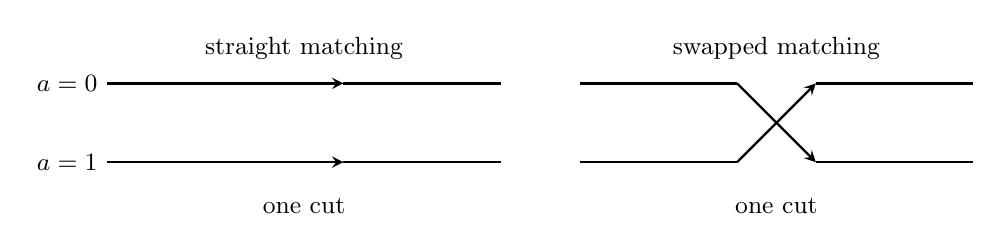
\begin{tikzpicture}[x=1cm,y=1cm,>=stealth,every node/.style={font=\small}]
\node at (2.5,1.45) {straight matching};
\draw[thick] (0,1)--(2,1);\draw[thick] (3,1)--(5,1);
\draw[thick] (0,0)--(2,0);\draw[thick] (3,0)--(5,0);
\draw[->,thick] (2,1)--(3,1);\draw[->,thick] (2,0)--(3,0);
\node[left] at (0,1) {$a=0$};\node[left] at (0,0) {$a=1$};
\node at (8.5,1.45) {swapped matching};
\draw[thick] (6,1)--(8,1);\draw[thick] (9,1)--(11,1);
\draw[thick] (6,0)--(8,0);\draw[thick] (9,0)--(11,0);
\draw[->,thick] (8,1)--(9,0);\draw[->,thick] (8,0)--(9,1);
\node at (2.5,-.55) {one cut};\node at (8.5,-.55) {one cut};
\end{tikzpicture}
\caption{The two allowed matchings at a cut. There are two independently
switchable cuts on the doubled time circle. Four Haar bundles keep the
integration space fixed throughout the interpolation.}
\label{cl:fig:seams}
\end{figure}

\begin{proposition}[exact replica response]\label{cl:prop:replica}
Let $\operatorname{Cov}_{u,v}$ denote covariance for the probability law
in \eqref{cl:eq:replica-F}. Then
\begin{equation}\label{cl:eq:replica-covariance}
2\psi_s(T)=\int_0^1\!\int_0^1
          \operatorname{Cov}_{u,v}(\Delta_c,\Delta_{c'})\,du\,dv.
\end{equation}
Write $\Delta_c=\sum_x A_x$ and $\Delta_{c'}=\sum_y B_y$, assigning
the three directions and two sheets at each cut to their bottom site.
The quantity
\[
I_{b,s,T}=\int_0^1\!\int_0^1\sum_{y\in s}
                  \operatorname{Cov}_{u,v}(A_0,B_y)\,du\,dv
\]
satisfies $\psi_s(T)=VI_{b,s,T}/2$. In particular, on $s=(2T)^3$,
the datum \Mcirc{} is equivalent to
\begin{equation}\label{cl:eq:replica-target}
I_{b,(2T)^3,T}\le\frac1{16388T^3}.
\end{equation}
\end{proposition}
\begin{proof}
At finite volume the exponent and its derivatives are bounded on the
compact integration space. Differentiating under the integral gives
$\partial_u\partial_vF=\operatorname{Cov}_{u,v}(\Delta_c,\Delta_{c'})$.
The fundamental theorem of calculus and \eqref{cl:eq:replica-corners}
give
\[
\int_{[0,1]^2}\partial_u\partial_vF
=F(1,1)-F(1,0)-F(0,1)+F(0,0)
=4\log Z(s,T)-2\log Z(s,2T)=2\psi_s(T).
\]
The interpolating measure is invariant under spatial translations, so
$\sum_{x,y}\operatorname{Cov}(A_x,B_y)
=V\sum_y\operatorname{Cov}(A_0,B_y)$. This proves the second identity.
For the cube $V=8T^3$, it reads $\psi=4T^3I$; multiplication by
$4097$ gives \eqref{cl:eq:replica-target}.
\end{proof}

The target is a signed integrated covariance bound.\footnote{An absolute
covariance bound would suffice, but it is stronger: the exact identity
permits cancellations both in space and in the interpolation parameters.}
It is not supplied by boundedness of the action. Indeed $|A_x|,|B_y|\le12b$,
because a cut has six plaquettes per bottom site and the difference of
two real traces is at most $4$. Cauchy--Schwarz therefore gives only
$|\operatorname{Cov}(A_x,B_y)|\le144b^2$ and
$|I_{b,s,T}|\le144b^2V$. This grows with the volume, whereas
\eqref{cl:eq:replica-target} decreases as $T^{-3}$.

\subsection{An exact conditional trace factorisation}
There is a second formulation that uses the vacuum measure of the
finite-volume transfer operator. Let $h>0$ be its unit Perron eigenvector,
let $R=\mathbb T/\lambda_0$, and put $\pi(dx)=h(x)^2dx$.
The Markov operator $P=h^{-1}Rh$ is reversible on $L^2(\pi)$.
For an integer $t\ge1$ let $p_t(x,y)$ be the transition density of $P^t$
relative to $\pi$. The kernel is continuous and positive at fixed volume,
so all conditional densities below are defined and finite. Unitary
equivalence and the Hilbert--Schmidt identity give
\begin{equation}\label{cl:eq:chi-trace}
\operatorname{Tr}R^{2t}=\int p_t(x,y)^2\,\pi(dx)\pi(dy).
\end{equation}
Partition the terminal links into $k$ blocks and write $y=(y_1,\ldots,y_k)$.
Let $\ell_j$ be the density of the conditional distribution of $y_j$ under
$P^t(x,dy)$, given $y_1,\ldots,y_{j-1}$, relative to the corresponding
conditional distribution under $\pi$. For each history, this density has
mean one. Set
\[
\chi_j^2(x,y_{<j})=\int(\ell_j-1)^2\,\pi(dy_j\mid y_{<j}),\qquad
S_j=\mathbb E_{\pi\otimes\pi}\prod_{i=1}^j\ell_i^2,
\quad S_0=1.
\]
The conditional-density chain rule gives $\prod_{j=1}^k\ell_j=p_t(x,y)$.
Let $\theta_{j-1}$ be the probability measure on $(x,y_{<j})$ with density
$S_{j-1}^{-1}\prod_{i<j}\ell_i^2$ relative to their
$\pi\otimes\pi$ marginal. Integrating the next block gives
\begin{equation}\label{cl:eq:chi-chain}
\frac{S_j}{S_{j-1}}=1+\mathbb E_{\theta_{j-1}}\chi_j^2,
\qquad
\log\operatorname{Tr}R^{2t}
=\sum_{j=1}^k\log\bigl(1+\mathbb E_{\theta_{j-1}}\chi_j^2\bigr).
\end{equation}
In fact $\int\ell_j^2\,d\pi(\cdot\mid y_{<j})=1+\chi_j^2$;
substitution into $S_j$ proves the first equality, and telescoping with
\eqref{cl:eq:chi-trace} proves the second.

For an even $T=2t$, estimates
\begin{equation}\label{cl:eq:chi-target}
\mathbb E_{\theta_{j-1}}\chi_j^2\le\frac1{8194k}
\quad(1\le j\le k)
\end{equation}
would imply $X_s(T)\le1/8194$, since $\log(1+x)\le x$ for $x\ge0$.
Consequently $\psi_s(T)\le2X_s(T)\le1/4097$.
The measure $\theta_{j-1}$ is essential: an estimate under the untilted
stationary law does not give \eqref{cl:eq:chi-target}.
For an explicit comparison, take the uniform law on four states
$x=(x_1,x_2)\in\{0,1\}^2$ and the reversible transition matrix
$P=\theta I+(1-\theta)J$, where $J(x,y)=1/4$ and $0<\theta<1$.
Reveal the terminal bits in order. Then
$\ell_1=1+\theta$ if $y_1=x_1$, and $\ell_1=1-\theta$ otherwise,
so $S_1=1+\theta^2$. On a matching first-bit history, the two possible
second-bit likelihoods are $1\pm2\theta/(1+\theta)$; on a mismatching
history both are one. Consequently
\[
\mathbb E_{\pi\otimes\pi}\chi_2^2
=\frac{2\theta^2}{(1+\theta)^2},\qquad
\mathbb E_{\theta_1}\chi_2^2
=\frac{(1+\theta)^2}{2S_1}
                       \frac{4\theta^2}{(1+\theta)^2}
=\frac{2\theta^2}{1+\theta^2}.
\]
For $\theta=1/3$ these means are $1/8$ and $1/5$, respectively.
The matrix has eigenvalues $1,\theta,\theta,\theta$, hence
$S_2=\operatorname{Tr}P^2=1+3\theta^2$ and
$S_2/S_1=1+\mathbb E_{\theta_1}\chi_2^2$ as required.
Equations \eqref{cl:eq:replica-target} and \eqref{cl:eq:chi-target}
are concrete analytical targets for the actual Wilson measures.
Neither is established here along the four-dimensional continuum tuning.
